\chapter{Methodology} \label{chap:Methodology}

\section{Software Development Life Cycle (SFLC)}

The methodology selected for this project was a mixture of the
incremental and iterative software development lifecycles. This
is a typical methodology selected for machine learning projects
as the exploratory nature of many machine learning projects
necessitates a management method which allows for the flexible
changing of approaches throughout the course of the project.

At a high level, the project is managed using an incremental
approach whereby I found promising ideas from my on-going
literature review and personal exploration of the EMG silent
speech dataset.

Then when I found an approach which I believed was promising,
I conducted initial small-scale experiments to either validate
or disprove my initial assumption, and then scaled up my experiments
iteratively to verify whether or not my hypothesis was valid.

The evaluation metric for each incremental approach was selected
based on the common evaluation metric for that task as reported
in the literature.

\section{Research Plan}

The research plan for my project is orignally based on my
Project Intiation Document (PID), but was modified as the 
data acquisition task for this project was cancelled.

The original research plan was based around finding improvements
to silent speech methods by using the Digital Voicing dataset
(\cite{gaddy2020digital}) open-source dataset and using the
data acquired from myself and participants. Unfortunately due
to financial constraints on the project and the difficulty in
acquiring the EMG data acquisition device which was originally
proposed in the PID, this objective of the project was no
longer achievable. The original project plan was segmented
based along two of the stated objectives of this project,
create an improved model / method for silent speech and data
acquisition.

\begin{center}
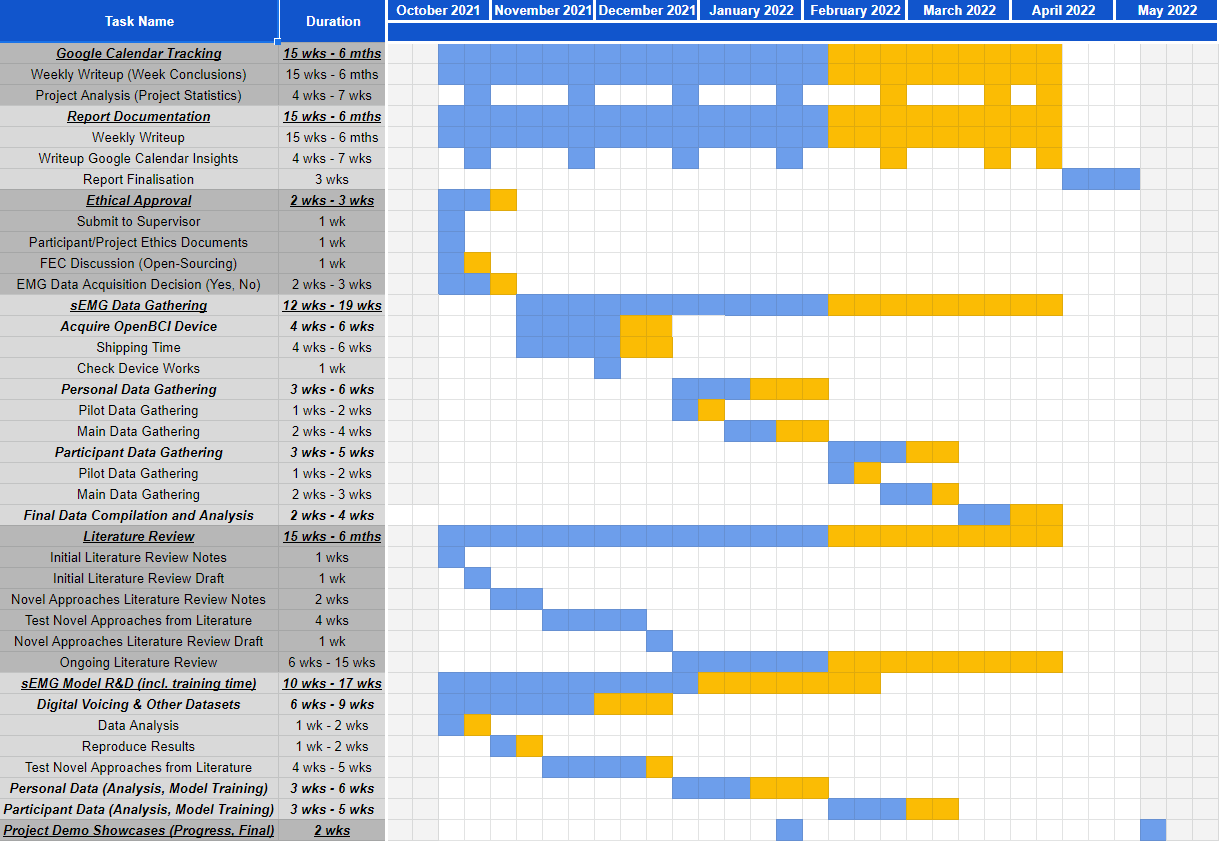
\includegraphics[scale=0.3]{graphics/planning/original_plan.png}
\end{center}

As I only decided to not pursue one of these objectives and
the main objective of my project was still attainable, I
simply stuck to the original project plan and allocated more
time to the research and development for silent speech
methods.

A timeline of major project milestones is provided in the
appendix for an overview of how the project was conducted.